
\documentclass[%
 %reprint,
%superscriptaddress,
%groupedaddress,
%unsortedaddress,
%runinaddress,
%frontmatterverbose, 
preprint,
%showpacs,preprintnumbers,
%nofootinbib,
%nobibnotes,
%bibnotes,
 amsmath,amssymb,
 aps,
%pra,
%prb,
%rmp,
%prstab,
%prstper,
%floatfix,
]{revtex4-1}

\usepackage{listings}
\usepackage{asymptote}
\usepackage{graphicx}% Include figure files
\usepackage{dcolumn}% Align table columns on decimal point
\usepackage{bm}% bold math
%\usepackage{hyperref}% add hypertext capabilities
%\usepackage[mathlines]{lineno}% Enable numbering of text and display math
%\linenumbers\relax % Commence numbering lines

%\usepackage[showframe,%Uncomment any one of the following lines to test 
%%scale=0.7, marginratio={1:1, 2:3}, ignoreall,% default settings
%%text={7in,10in},centering,
%%margin=1.5in,
%%total={6.5in,8.75in}, top=1.2in, left=0.9in, includefoot,
%%height=10in,a5paper,hmargin={3cm,0.8in},
%]{geometry}
\usepackage[margin=25mm]{geometry}
\usepackage{changepage}
\usepackage{mathcomp}
\usepackage[english]{babel}
\usepackage{siunitx}
\usepackage{tikz}
\DeclareSIUnit\minute{min}
\usepackage{amsmath,mathrsfs,amsfonts,amssymb,amsthm } %permette di mettere formule una sotto l'altra,
%dovrebbe scrivere lettere corsive eleganti con "\mathscr{--},"
% permette di definire insiemi numerici con \mathbb{""},
\usepackage[utf8]{inputenc} %accenti
\theoremstyle{plain} 
\theoremstyle{definition}
\newtheorem{defn}{Def}[section]
\theoremstyle{plain}
\newtheorem{thm}{Theorem}[section] 
\newcommand{\R}{\mathbb{R}}
\newcommand{\N}{\mathbb{N}}
\newcommand{\off}{\text{off}}
\newcommand{\mat}{\text{Mat}}
\newcommand{\B}{\mathbf{B}}
\newcommand{\A}{\mathbf{A}}
%\newcommand{\S}{\mathbf{S}}
\newcommand{\open}{\left}
\newcommand{\close}{\right}
\newcommand{\void}{\varnothing}
\newcommand{\xslash}{\setminus}

%\newcommand{\fnorm}{\lVert #1 \rVert_F}

\usepackage[T1]{fontenc}
\usepackage{subfig}
\usepackage{caption}
\usepackage{subfig}
\usepackage{booktabs}
\usepackage{float}
\usepackage{mathdots}
\usepackage{mathrsfs}
\usepackage{braket}
\usepackage{hyperref}
\usepackage{float}
\usepackage{gensymb}

\usepackage{pgfplots}
\usepackage{circuitikz}
\usepackage{hyperref}
\usepackage{tkz-tab}
\usepackage{caption}
\usetikzlibrary{backgrounds,automata}
\pgfplotsset{/pgf/number format/use comma,compat=newest}
\usetikzlibrary{graphs,shapes,positioning,shadows}

\usepackage{colortbl}
\newcommand{\blue}[1]{\textcolor{blue}{#1}}
\newcommand{\red}[1]{\textcolor{red}{#1}}
\newcommand{\green}[1]{\textcolor{green}{#1}}
\newcommand{\magenta}[1]{\textcolor{magenta}{#1}}
\newcommand{\cyan}[1]{\textcolor{cyan}{#1}}
\newcommand{\yellow}[1]{\textcolor{yellow}{#1}}
\newcommand{\grey}[1]{\textcolor{grey}{#1}}
\newcommand{\abs}[1]{\lvert#1\rvert}

\begin{document}


\title{FYS 3150 - Project 3}% Force line breaks with \\
%\thanks{A footnote to the article title}%


\author{Lorenzo Speri}
\affiliation{University of Oslo, Department of Physics}
%
% Authors' institution and/or address\\
% This line break forced with \textbackslash\textbackslash
%}%

%\collaboration{CLEO Collaboration}%\noaffiliation

\date{\today}% It is always \today, today,
             %  but any date may be explicitly specified
\maketitle

\begin{center}
\section{Abstract}
We use a two-dimensional Ising model to simulate a lattice of spins that undergoes a phase transition. Assuming a canonical ensemble we relate physical quantities to the configurations of the system for different temperatures. The behavior of the possible energy configurations is studied linking the microstates and the phase transitions. We estimate a critical temperature for different lattice dimension also discussing the limit of our model. We find approximatley how many Monte Carlo trials our system needs to reach an equilibrium state $n \approx 5 \times 10^4$ at different temperatures. In addition the Metropolis algorithm is explained and implemented in the code.
\end{center}

%\begin{description}
%\item[Usage]
%Secondary publications and information retrieval purposes.
%\item[PACS numbers]
%May be entered using the \verb+\pacs{#1}+ command.
%\item[Structure]
%You may use the \texttt{description} environment to structure your abstract;
%use the optional argument of the \verb+\item+ command to give the category of each item. 
%\end{description}

\begin{itemize}
\item URL to GitHub folder of the code: \url{https://github.com/lorenzsp/Project4.git}
\end{itemize}


%\pacs{Valid PACS appear here}% PACS, the Physics and Astronomy
                             % Classification Scheme.
%\keywords{Suggested keywords}%Use showkeys class option if keyword
                              %display desired


%\tableofcontents
\section{Introduction}
%You don’t need to answer all questions in a chronological order. When you write the introduction you could focus on the following aspects
%Motivate the reader, the first part of the introduction gives always a motivation and tries to give the overarching ideas
%What I have done
%The structure of the report, how it is organized etc
A phase transition in a magnetic system is an important physical process which can be studied with the so-called Ising model. For example a ferromagnetic material presents an ordering phenomenon at the atomic level which causes the unpaired electron spins to line up parallel. But after a certain temperature the magnetization of the ferromagnetic material disappears. We want to simulate this phenomenon considering a $L\times L$ lattice and we implement a code with the Ising model in two dimensions and periodic boundary conditions (PBC). The physical quantities we study with the simulation are: the mean energy $<E>$, the mean absulute value of magnetizaiton $<|M|>$, the specific heat $C_v$ and the susceptibility $\chi$. The code for the numerical experiments is explained and as a consequence we also discuss Metropolis' algorithm. We give also a motivation to parallelize the code. \\
At first a $2 \times 2$ lattice is studied and the numerical results are compared with the analytical expressions for different values of temperature. After using this case as a benchmark for our code, we increase the lattice dimension up to $L=20$. At different temperatures the behavior of the mean energy and absolute vlaue of magnetisation is studied as a function of the Monte Carlo cycles. \\
The probability distribution of the energy is also analyzed and a physical explanation of the system is given. \\
A phase transition is marked by abrupt macroscopic changes as temperature changes. The Ising model exhibits a second-order phase transition since the heat capacity and susceptibility diverge for a specific $T_C$. We study $\chi$ and $C_v$ with different dimensions of the lattice in order to extract a value of $T_C$. 

\section{Methods and algorithms}
%Describe the methods and algorithms
%You need to explain how you implemented the methods and also say something about the structure of your algorithm and present some parts of your code
%You should plug in some calculations to demonstrate your code, such as selected runs used to validate and verify your results. The latter is extremely important!! A reader needs to understand that your code reproduces selected benchmarks and reproduces previous results, either numerical and/or well-known closed form expressions.
\subsection{Description of the model and hypothesis}
We want to make a two dimensional model for studying a magnetic material. Our model is a lattice of dimension $L \times L$ where we neglect any quantum mechanical behavior. We also assign a magnetic moment to each lattice site. We consider a binary system where each magnetic moment $k$ can only take on two values: spin up or down respectivley $s_k=+1=\, \uparrow$ or $s_k=-1=\, \downarrow$. A configuration of our lattice can be represented as:
\begin{equation} \notag
\begin{array}{cccc}
\uparrow & \downarrow & \downarrow  & \cdots \\
\downarrow & \uparrow & \downarrow & \cdots \\
\downarrow & \uparrow & \uparrow &  \cdots \\
\vdots & \vdots & \vdots &  \\
\end{array}
\end{equation}
The total magnetic moment (or magnetizationis) is defined by the sum of all the spins in the lattice:
\begin{equation}
M = \sum_{k=1} ^N s_k
\end{equation}
where we do not consider the units of this quantity.
According to Ising model we express the energy of a possible configuration of the system without any externally applied magnetic field as:
\begin{equation}
\label{energy}
E = -J \, \sum_{<k \, l>} ^N s_k \, s_l
\end{equation}
where $J$ is a constant expressing the strength of the interaction between neighboring spins, $<k \, l>$  indicates that we sum over nearest neighbors only, and $N$ is given by the total number of spins. In the model we use periodic boundary conditions (PBC) that can be represented as in Figure(\ref{PBC}),also the spins at the border interact with four neighbors.
\begin{figure}
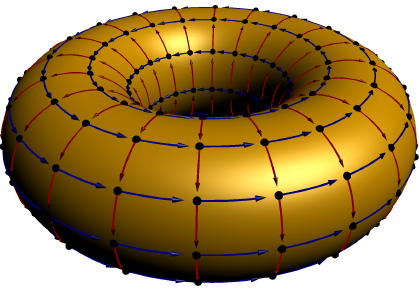
\includegraphics[scale=0.5]{torus}
\caption{Graphical representation of periodic boundary conditions (PBC), each dot in the figure represents a spin configurations}
\label{PBC}
\end{figure}
We also assume that our system is a canonical ensemble where temperature $T$ is an external parameter. The possible energy and magnetization configurations $E_i$ and $M_i$ are microstates that are distributed according to Boltzmann distribution:
\begin{equation}
\label{boltzmann_pdf}
P_i(T) = \frac{e^{-\beta \, E_i}}{Z} \hspace{0.5cm} \beta = \frac{1}{k_B \, T}
\end{equation}
where $k_B$ is the Boltzmann constant and $Z$ is the partition function:
\begin{equation}
Z = \sum_{i} ^m \, e^{-\beta \, E_i }
\end{equation}
$m$ represents the number of all possible configurations, in our case $m=2^{L \times L}$.
We can now define the mean value of the energy and its variance as:
\begin{align}
<E> &= \frac{1}{Z} \, \sum_i \, E_i \, e^{-\beta \, E_i} = - \, \left(\frac{\partial \, \ln{Z}}{\partial \beta} \right) \\
\sigma^2_E &= <E^2> - <E>^2 
\end{align}
In the same way we can define the mean value of the magnetization and its variance.
In our case we define the heat capacity as:
\begin{equation}
\label{heat}
C_v = \frac{1}{k_B T^2} \, (<E^2> - <E>^2 )
\end{equation}
while the susceptibility is defined as:
\begin{equation}
\label{chi}
\chi = \frac{1}{k_B T} \, (<M^2> - <M>^2 )
\end{equation}
The Ising model in two dimensions (in the limit $L \to \infty$) undergoes a phase transition of second order, this means that below a given critical temperature $T_C$, the model exhibits a spontaneous magnetization with $<M>  \neq 0$. Above $T_C$ the average magnetization is zero. The mean magnetization approaches zero at $T_C$ with an infinite slope. Such a behavior is an example of what are called critical phenomena. The point where a phase transition occurs is called a critical point. This point is given by the temperature $T_C$ where $C_v$ and $\chi$ diverge and the megnetization disappears. 
\subsection{Code implementation and Metropolis algorithm}
The model of our lattice is implemented using a matrix of dimension $L \times L$ where each element represents a spin up $=+1$ or down $=-1$.
We set an initial configuration for the spin matrix and calculate the initial value of energy and magnetization. Periodic boundary conditions are implemented using the following function that returns the proper index.
\lstset{numbers=none, numberstyle=\tiny, stepnumber=2, numbersep=5pt}
\begin{lstlisting}
inline int periodic(int i, 
    int limit, int add) {
    return (i+limit+add) % (limit);
}
\end{lstlisting}
We now define what is known as a Monte Carlo experiment (or trial):
\begin{itemize}
\item perform a double loop over all spins of the lattice 
\lstset{numbers=none, numberstyle=\tiny, stepnumber=2, numbersep=5pt}
\begin{lstlisting}
    for(int x=0; x<lattice_dim; x++){
        for(int y=0; y<lattice_dim; y++){
\end{lstlisting}
\item selcet a random position in the lattice, i.e. we choose two random indeces $[xr][yr]$ in the spin matrix using $mt19937\_64$ random generator
\item flip the spin in the lattice site $[xr][yr]$
\item calculate the energy difference $\Delta E$ from the previous configuration
\item using Metropolis algorithm we decide to accept or not the new configuration
\item update values

\item end the loop over all spins

\end{itemize}
This will be repeated as many times as possible to get a good approximation for the expectation values. From a physical point of view the loop over all spins is crucial because we need to give to all the spins the possibility to be changed. Otherwise, the expectation values will be correlated. If we are interested in the evolution of the system as a function of the temperature we need only to add another loop over the interested temperature range.\\
It is possible to precalculate the energy difference in order to reduce the running time. In fact, there are only five possibilities:
\begin{itemize}
\item[1)] $\Delta E=8J$
\[
\begin{array}{ccc}
 		& \uparrow & \\
\uparrow & \uparrow & \uparrow  \\
		   & \uparrow &  \\
\end{array}
\hspace{0.5cm}
\Rightarrow
\hspace{0.5cm}
\begin{array}{ccc}
 		& \uparrow & \\
\uparrow & \downarrow & \uparrow  \\
		   & \uparrow &  \\
\end{array}
\]
\item[2)] $\Delta E=4J$
\[
\begin{array}{ccc}
 		& \uparrow & \\
\downarrow & \uparrow & \uparrow  \\
		   & \uparrow &  \\
\end{array}
\hspace{0.5cm}
\Rightarrow
\hspace{0.5cm}
\begin{array}{ccc}
 		& \uparrow & \\
\downarrow & \downarrow & \uparrow  \\
		   & \uparrow &  \\
\end{array}
\]
\item[3)] $\Delta E=0$
\[
\begin{array}{ccc}
 		& \uparrow & \\
\downarrow & \uparrow & \uparrow  \\
		   & \downarrow &  \\
\end{array}
\hspace{0.5cm}
\Rightarrow
\hspace{0.5cm}
\begin{array}{ccc}
 		& \uparrow & \\
\downarrow & \downarrow & \uparrow  \\
		   & \downarrow &  \\
\end{array}
\]
\item[4)] $\Delta E=-4J$
\[
\begin{array}{ccc}
 		& \downarrow & \\
\downarrow & \uparrow & \uparrow  \\
		   & \downarrow &  \\
\end{array}
\hspace{0.5cm}
\Rightarrow
\hspace{0.5cm}
\begin{array}{ccc}
 		& \downarrow & \\
\downarrow & \downarrow & \uparrow  \\
		   & \downarrow &  \\
\end{array}
\]
\item[5)] $\Delta E=-8J$
\[
\begin{array}{ccc}
 		& \downarrow & \\
\downarrow & \uparrow & \downarrow \\
		   & \downarrow &  \\
\end{array}
\hspace{0.5cm}
\Rightarrow
\hspace{0.5cm}
\begin{array}{ccc}
 		& \downarrow & \\
\downarrow & \downarrow & \downarrow  \\
		   & \downarrow &  \\
\end{array}
\]
\end{itemize}
We now explain the Metropolis algorithm applied to our case.
At a fixed temperature a new configuration $E_b$ is generated from a previous one $E_a$ using a transition probability $W(a\to b)=R(a\to b) A(a\to b)$. $R(a\to b)$ is the likelihood of making the transition and contains all the information about our system, while $A(a\to b)$ is the probability of accepting the move from $a$ to $b$. According to Markov chain theory the detailed balance condition is given by:
\begin{equation}
\label{detailed_balance}
\frac{P_b}{P_a} = \frac{W(a\to b)}{W(b\to a)} = \frac{R(a\to b) A(a\to b)}{R(b\to a) A(b\to a)}
\end{equation}
We assume the probability of picking a given spin $R(b\to a)$ as a uniform distribution, so using the Boltzmann distribution (\ref{boltzmann_pdf}) we can rewrite equation(\ref{detailed_balance}) as:
\[
\frac{e^{-\beta \, E_b}}{e^{-\beta \, E_a}} = \frac{A(a\to b)}{A(b\to a)}
\]
We need a model for the acceptance probability $A(a \to b)$ which allows every possible state of the system can be reached from any starting point if the simulations is carried out for a long enough time.We use the Metropolis-Hastings acceptance probability: we accept the move if the state is more likely, indeed $P_b/P_a >1$. If $P_b/P_a <1$ we pick a random number $r \in (0,1)$ and if $r\le P_b/P_a$ we accept the move otherwise we do not accept it. We implement this using the precalculated exponential of the energy differences $EnergyDifference$:
\begin{lstlisting}
if(distribution(gen) <= EnergyDifference[deltaE/4 + 2]){
spin_matrix[xr][yr] *= -1;
// update values
E += (double) deltaE;
M += (double) 2*spin_matrix[xr][yr];
}
\end{lstlisting}
\par 
When we perform the numerical experiment we use the following statistical estimator to find the expectation value of a quantity $B$:
\begin{equation}
<B> = \frac{1}{n} \, \sum_{l=1} ^n B_l
\end{equation}
where $n$ is the number of the Monte Carclo trials, and $B_l$ is one of the all outcome in the numerical experiment.
We make our considerations on each physical quantity assuming that $n$ tends to infinity. This assumption can be made if we have a large numeber of Monte Carlo cycles.\\
\begin{table}[h!]
\centering
\setlength{\tabcolsep}{12pt}
\caption{The table shows the running time when we parallelize a code or not. The code has calculated $<E>$, $<|M|>$, $\chi$, $C_v$ in a temperature range $T\in[2.2,2.3] \, kT/J$ with a temperature step size $dT = 0.005$ for different lattice dimension $L$}
\label{time}
\begin{tabular}{ccc}
\toprule
$L$ &  Parallelized code & Normal code \\
\midrule
  40	    &   2.18656 & 7.33698 \\
  60	     &  4.75809 & 17.0014 \\
  80	     &  8.43173 & 29.8397 \\
  100	 &  14.1064 & 46.9271 \\
\bottomrule
 & time in seconds & time in seconds
\end{tabular}

\end{table}
Parallelizing the code allows us to exploit more processors and to reduce the running time. Let us take an example of the running time needed to estimate $<E>$, $<|M|>$, $\chi$, $C_v$ in a temperature range $T\in[2.2,2.3] \, kT/J$ with a temperature step size $dT = 0.005$. 
We run the parallelized code with two processors with different lattice dimensions, so we have a total number of Monte Carlo cycles euqal to $2 \times 10^3$. We can notice from Table(\ref{time}) that we could get a better statistichs than the normal code with one third of the time


%\begin{equation}
%A(a \to b) = 
%\begin{cases}
%\exp(- \beta(E_b-E_a)) \hspace{0.5cm} if \quad E_b-%E_a>0 \\
%1 \hspace{0.5cm} else
%\end{cases}
%\end{equation}
%\setlength{\unitlength}{2pt}
%\begin{picture}(70,40)(0,-5)
%\newsavebox{\verticalfour} 
%\savebox{\verticalfour}(0,0)[bl]{
%	\multiput(0,0)(0,10){4}{\circle{2}}     % spins
%	\multiput(0,5)(0,10){4}{\line(0,-1){3}} % lines down
%	\multiput(0,-5)(0,10){4}{\line(0,1){3}} %   lines up
%	\multiput(2,0)(0,10){4}{\line(1,0){6}}  % lines right
%}
%\multiput(0,0)(10,0){6}{\usebox{\verticalfour}}
%\end{picture}
\pagebreak


\section{Results}
%Present your results
%Give a critical discussion of your work and place it in the correct context.
%Relate your work to other calculations/studies
%An eventual reader should be able to reproduce your calculations if she/he wants to do so. All input variables should be properly explained.
%Make sure that figures and tables should contain enough information in their captions, axis labels etc so that an eventual reader can gain a first impression of your work by studying figures and tables only.
We measure the energy in terms of the constant $J$. In the numerical experiments we set $k_B=1 \, J^2/kT$ so we define the unit of temperature $[T]= kT/J$ where $kT$ is the amount of heat required to increase the thermodynamic entropy of a system, in natural units, by one $nat=1/\ln(2)$. 
\subsection{$2\times 2$ lattice}
Let us consider a $2 \times 2$ lattice with periodic boundary conditions.
The energy of a configuration $i$ is given by:
\begin{equation}
\begin{split}
E_i = - J \, \sum _{<kl>} ^4 s_k s_l =\\
= - J ( s_1 s_2 + s_2 s_1 \\
 + s_1 s_3 + s_3 s_1 \\
 + s_3 s_4 + s_4 s_3 \\
 + s_2 s_4 + s_4 s_2 )
\end{split}
\end{equation}
So the possible configurations of energies and magnetization are $2^4 = 16$ and they are shown in Table(\ref{configurations})
\begin{table}
\centering
\setlength{\tabcolsep}{12pt}
\caption{Possible configurations of energy and magnetization for a lattice dimension $L=2$}
\label{configurations}
\begin{tabular}{cccc}
\toprule
Number of spin up & Degeneracy  & E & M \\
\midrule
4 & 1 & -8$J$  & 4 \\
3 & 4 &	 0 & 2 \\
2 & 4 & 0  & 0 \\
2 & 2 &  8$J$ & 0 \\
1 & 4 &  0 & -2   \\
0 & 1 & -8$J$ & -4 \\
\bottomrule
\end{tabular}

\end{table}
In this case we can calculate the partition function:
\[
Z = 2e^{-8J\beta} + 2e^{8J\beta} + 12 = 4 \cosh(8J\beta) + 12
\]
The mean value of the energy is given by:
\begin{equation} \notag
<E> = \sum _{i=1} ^{16} P_i E_i = - \frac{J}{Z} \, \left( 16 e^{8J\beta} - 16e^{-8J\beta} \right)
\end{equation}
and the mean of absulute value of the magnetization:
\begin{equation}
<|M|> = \sum _{i=1} ^{16} P_i |M_i| = \frac{1}{Z} \, \left( 8 e^{8J\beta} + 16 \right)
\end{equation}
while the mean value of magnetization can easily be found as $<M> = 0$. 
The the mean value of energy squared and magnetization squared are respectively:
\begin{equation}
\begin{split}
<E^2> =\frac{256}{Z} (\cosh(8J\beta)) \, J^2 \\
<M^2> =  \frac{1}{Z} (32e^{+8J\beta} + 32)
\end{split}
\end{equation}
using the equation (\ref{heat}) and (\ref{chi}) we can define the heat capacity and the susceptibility in our case:
\begin{equation}
\begin{split}
C_v = \frac{1024 +3072 \cosh(8J\beta)}{(4\, \cosh(8J\beta)+12)^2 \, k_B T^2} \\
\chi = \frac{(32e^{+8J\beta} + 32)}{(4\, \cosh(8J\beta)+12)} \, \frac{1}{\beta}
\end{split}
\end{equation}

\begin{figure}[h!]
\centering
     \subfloat[]{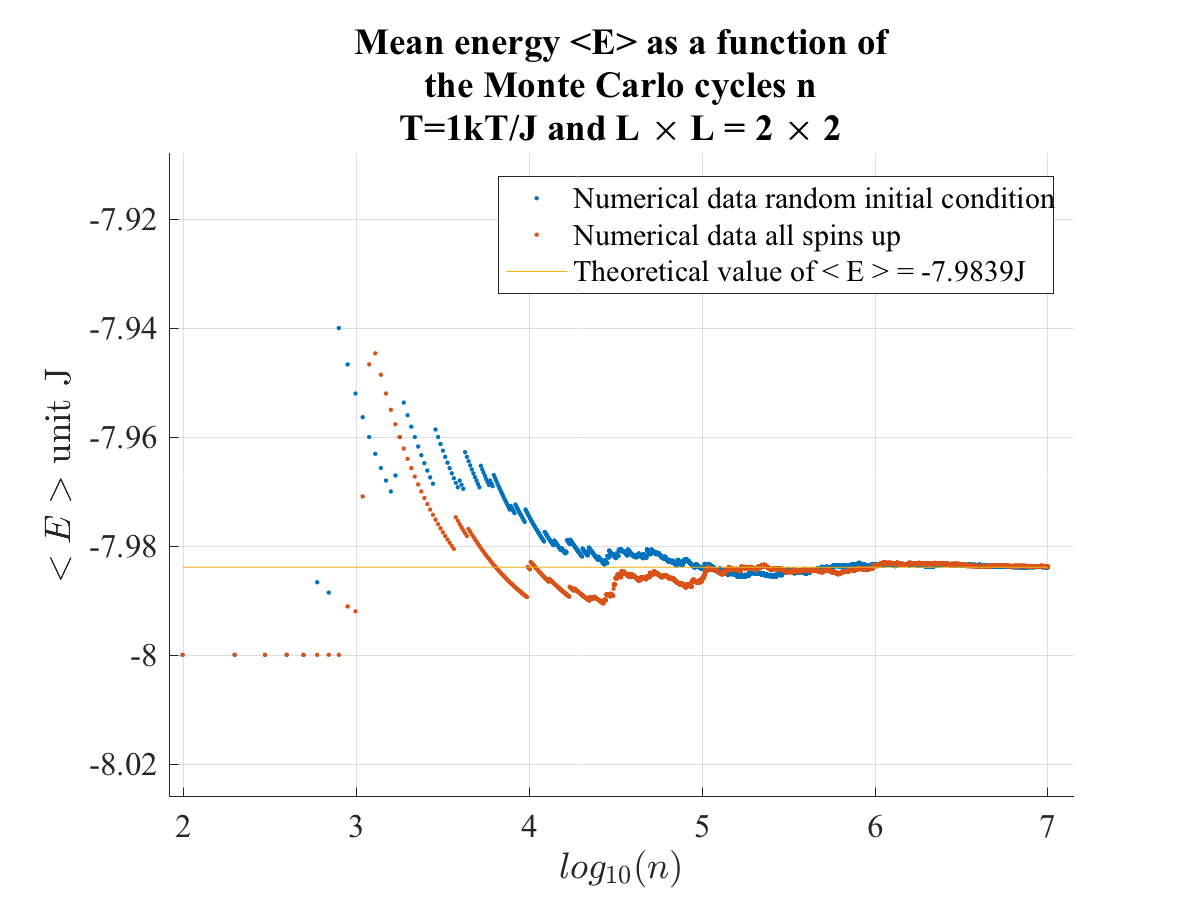
\includegraphics[width=.5\linewidth]{energy2x2.eps}\label{energy2x2}}
     \subfloat[]{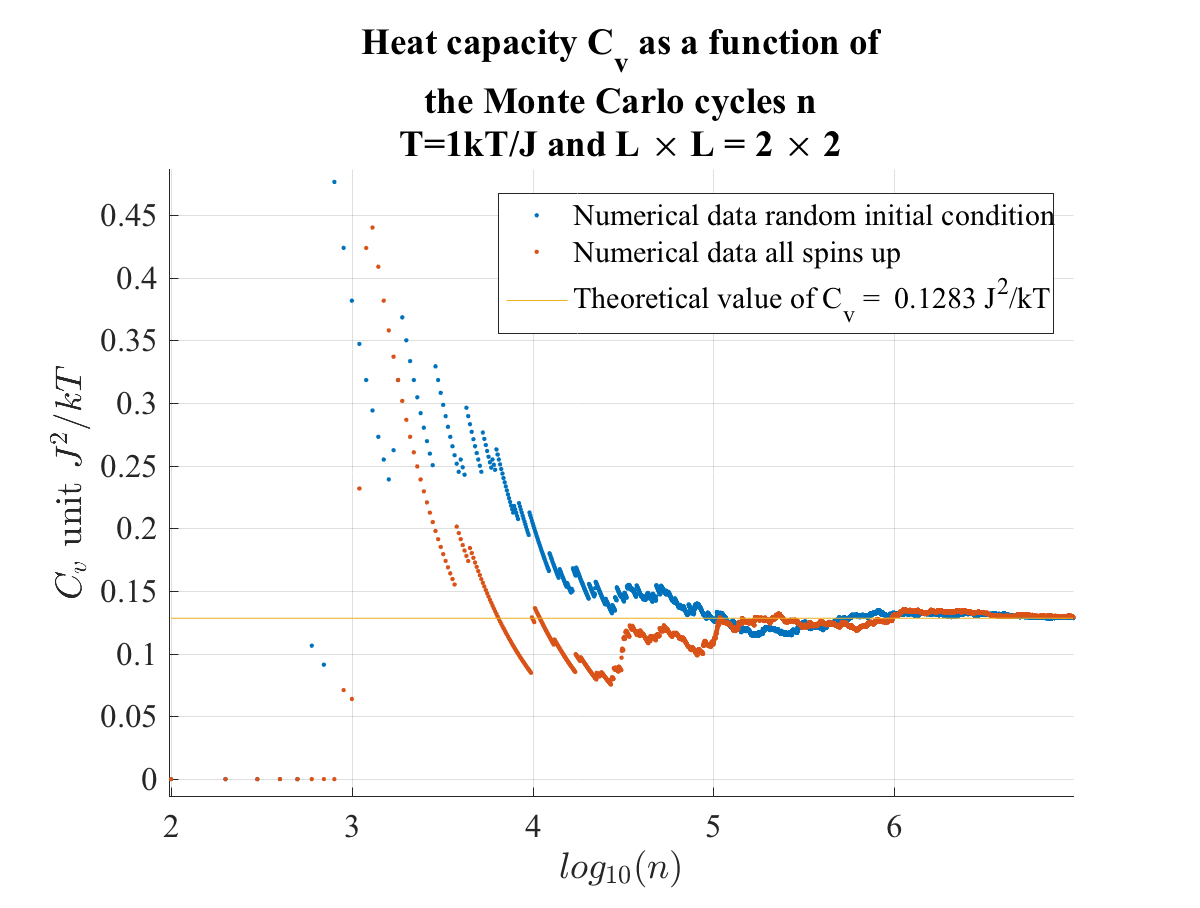
\includegraphics[width=.5\linewidth]{cv2x2.eps}\label{cv2x2}}
\caption{In Figure (a) and (b) are shown respectively mean energy and heat capacity as a function of Monte Carlo cycles $n$ for a temperature $T=1 kT/J$ and lattice dimension $L=2$. Both the quantities approach the theoretical value for $n \approx 10^5$}
\end{figure}
\begin{figure}[h]
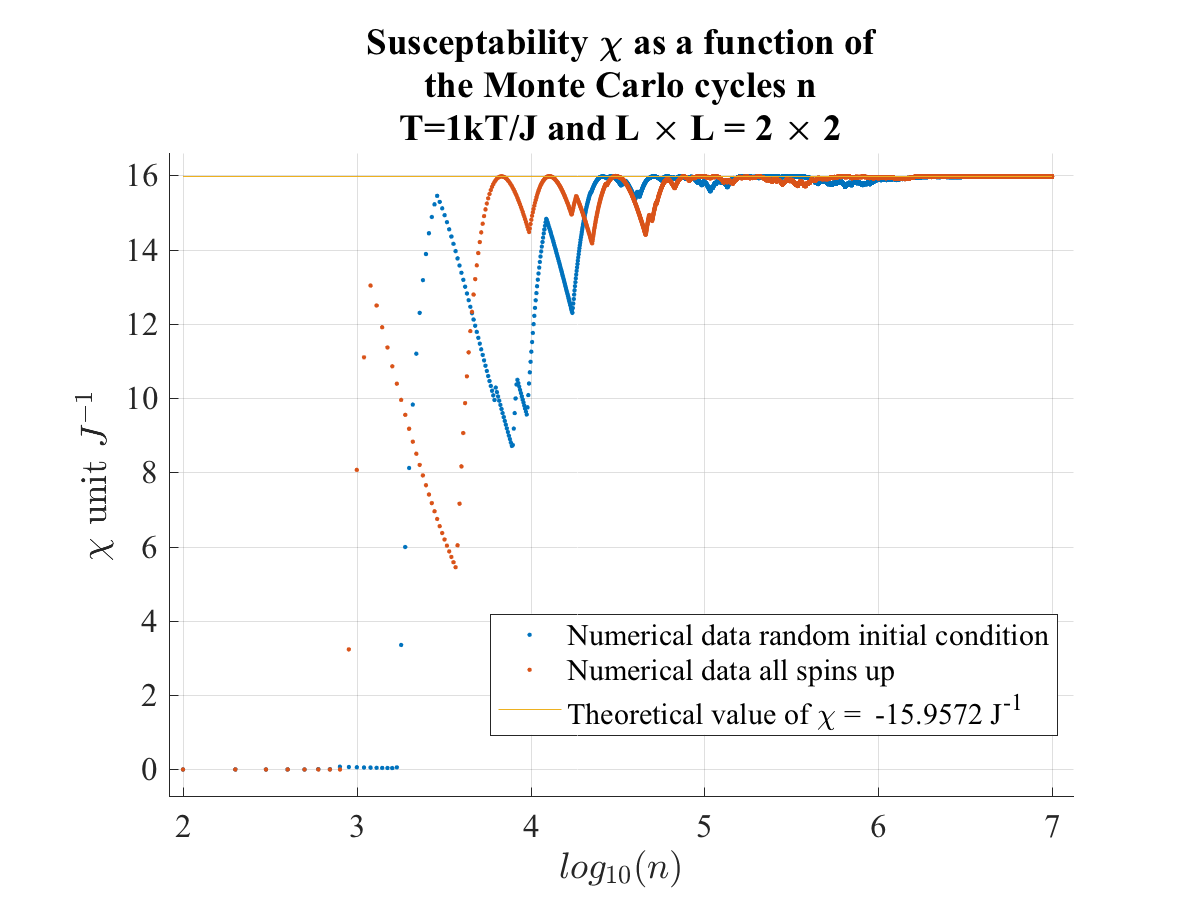
\includegraphics[scale=0.50]{chi2x2.eps}
\caption{The susceptibility of a lattice $L=2$ jumps under the theoretical value. This is due to the term $<|M|>$  in its formula.}
\label{chi2x2}
\end{figure}
We run $n=10^7$ Monte Carlo experiments and we study the behavoir of $<E>$, $<|M|>$, $C_v$, $\chi$ and $<M>$ as a function of $n$ at $T=1 \, kT/J$. We perform the same experiment with two initial configurations: first with a random initial positions of the spins and then with all spins up. We write to file the data when $n$ can be divided by 100: $n\%100==0$.\\
In Figures (\ref{energy2x2}) and (\ref{cv2x2}) notice that the most likely state is reached with good precision when $n \approx 10^{5}$ with both the initial conditions.
In Figure(\ref{absm2x2}) $<|M|>$ follows the same behavior of heat capaicity and energy, while the mean value of magnetization $<M>$ takes more Monte Carlo cycles before reaching the most likely state. 
\begin{figure}[h!]
\centering
     \subfloat[]{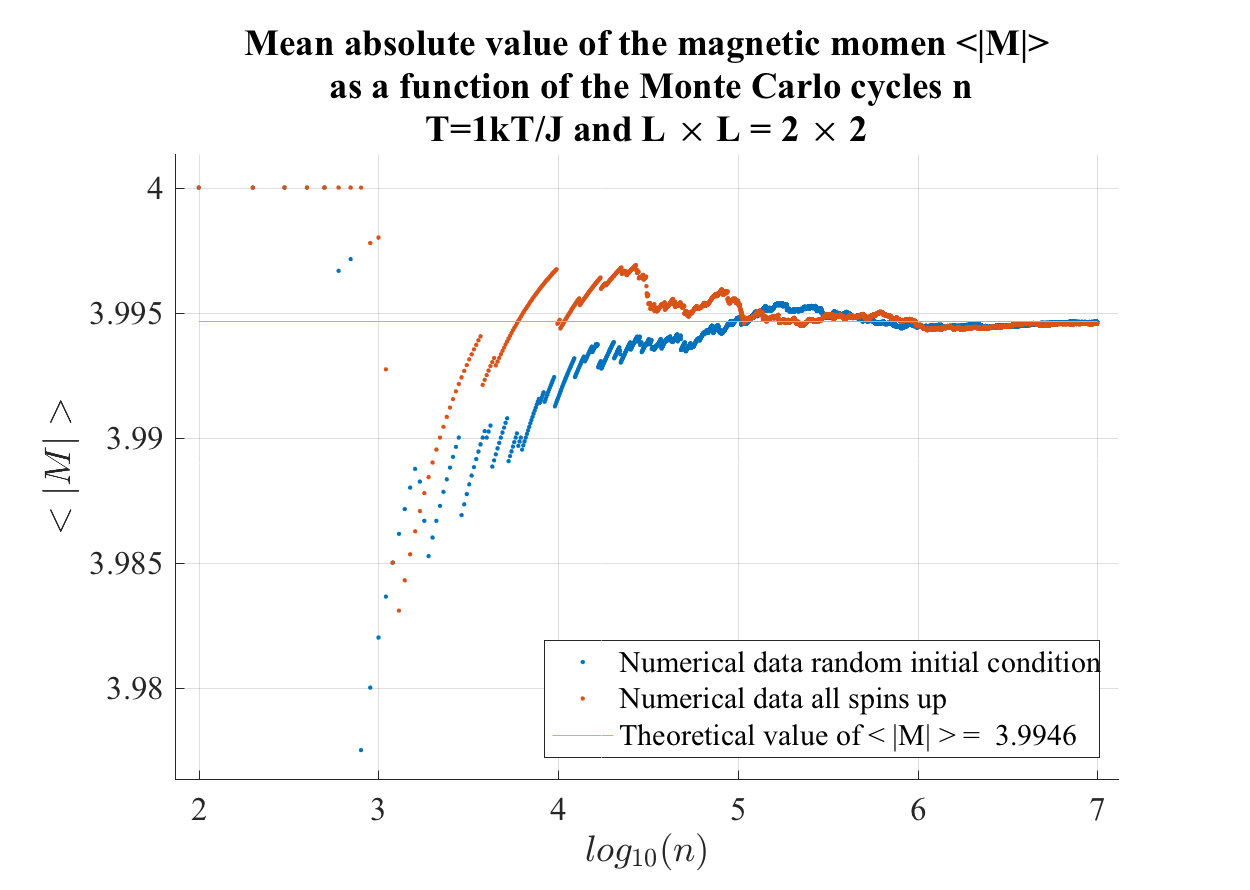
\includegraphics[width=.5\linewidth]{absm2x2.eps}\label{absm2x2}}
     \subfloat[]{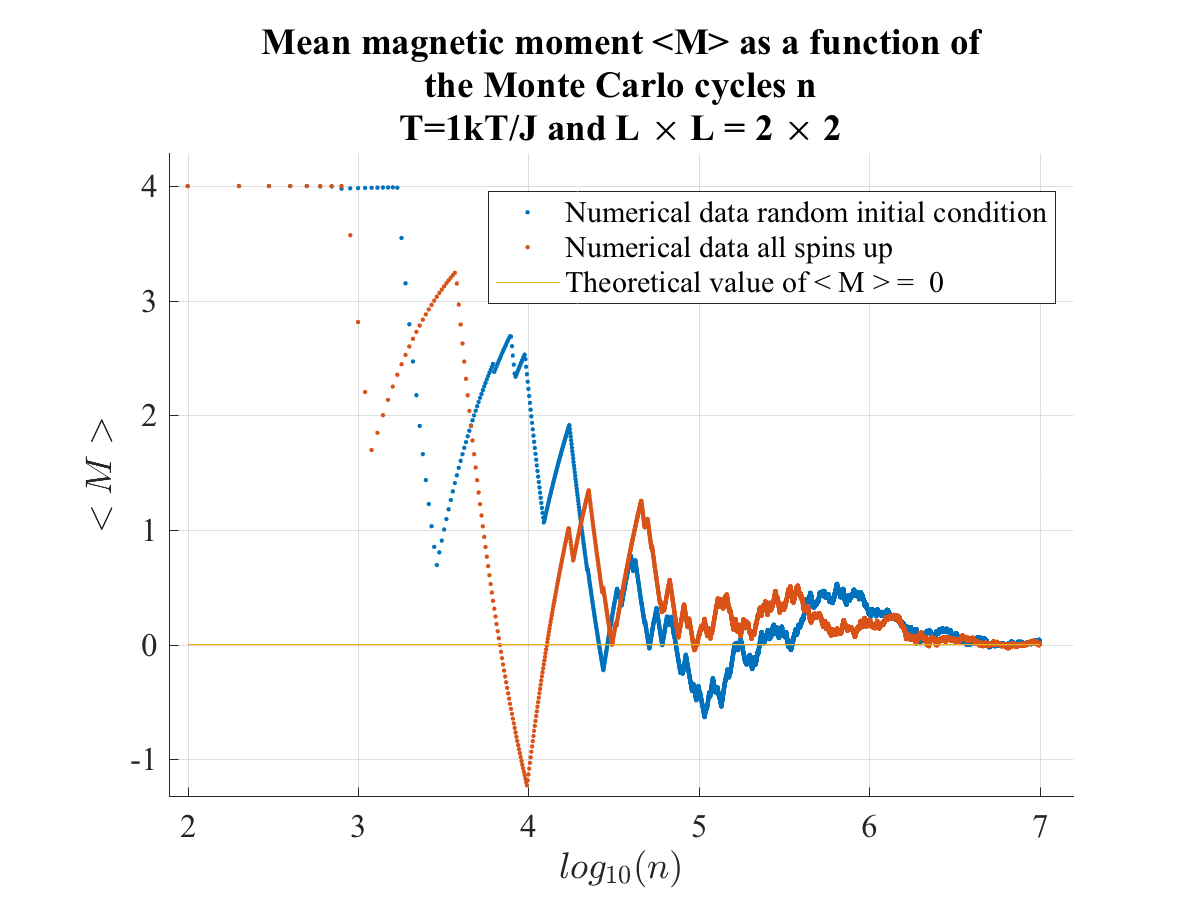
\includegraphics[width=.5\linewidth]{m2x2.eps}\label{m2x2.eps}}
\caption{In Figure (a) and (b) are shown respectively mean absulute value of magnetization and the mean magnetization as a function of Monte Carlo cycles $n$ for a temperature $T=1 kT/J$ and lattice dimension $L=2$. We can notice that the mean magnetization takes more Monte Carlo cycles before reching a steady state.}
\end{figure}


We now study a lattice $L \times L = 20 \times 20$ and we consider the behavior of the mean energy and mean absulute value of magnetization at different temperatures $T$. 
In Figure(\ref{e20x20}) shows that as temperature increases, the mean energy does as well. This reflects the physical phenomena that when a system is heated up its energy increases. Figure(\ref{absm20x20.eps}) we notice the magnetization decreases with temperature. Indeed, when the temperature is low the magnetic moment of each lattice tends to be aligned, while when the temperature increases the magnetization tends to zero. 
\begin{figure}[H]
\centering
     \subfloat[]{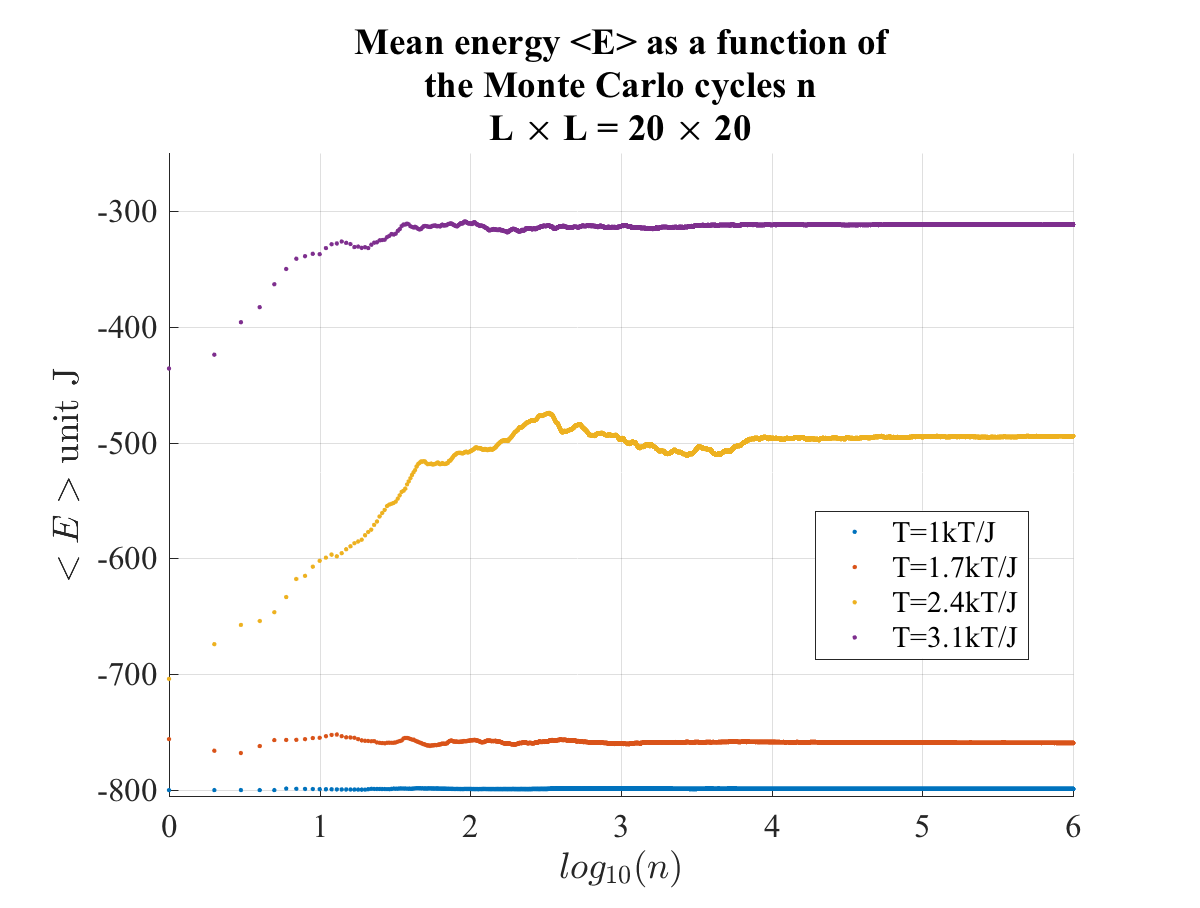
\includegraphics[width=.5\linewidth]{e20x20.eps}\label{e20x20}}
     \subfloat[]{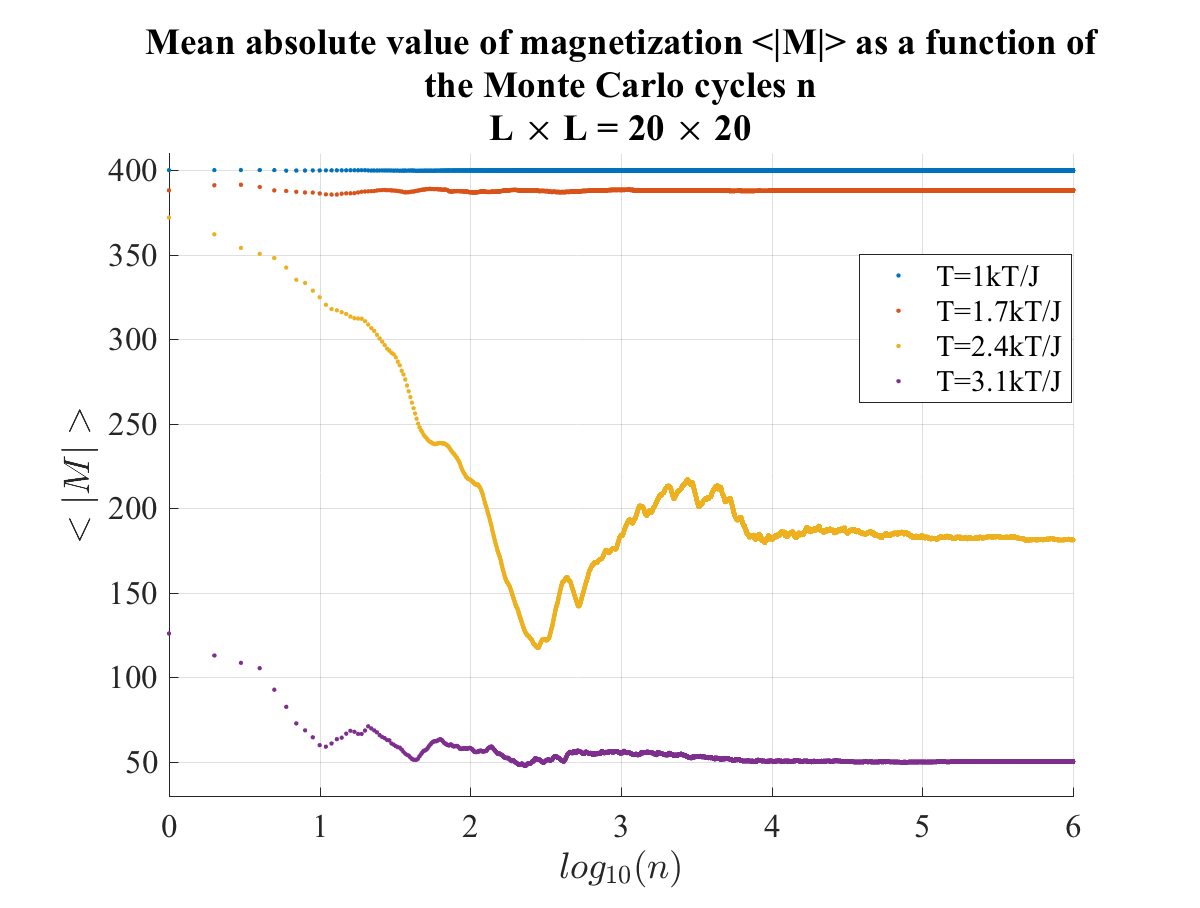
\includegraphics[width=.5\linewidth]{absm20x20.eps}\label{absm20x20.eps}}
\caption{In Figure (a) and (b) are shown respectively mean energy and mean absolute value of magnetization as a function of Monte Carlo cycles $n$ for different temperatures and lattice dimension $L=20$. At temperature $2.4 kT/J$ both the quantities take more time to reach a steady state.}
\end{figure}
We want to analyze the behavior of the system configurations at different temperatures and understand why the most unstable case is that with $T=2.4 \, kT/J$ for both magnetization and energy. To do that we calculate the probability density function $P(E)$ of the energy with $n=10^7$ Monte Carlo cycles. Taking into account the above considerations, we set a threshold of $n^* = 5 \time 10^4 $ over which we start writing to file data the number of times a given energy appears. \\
\begin{figure}[h]
\centering
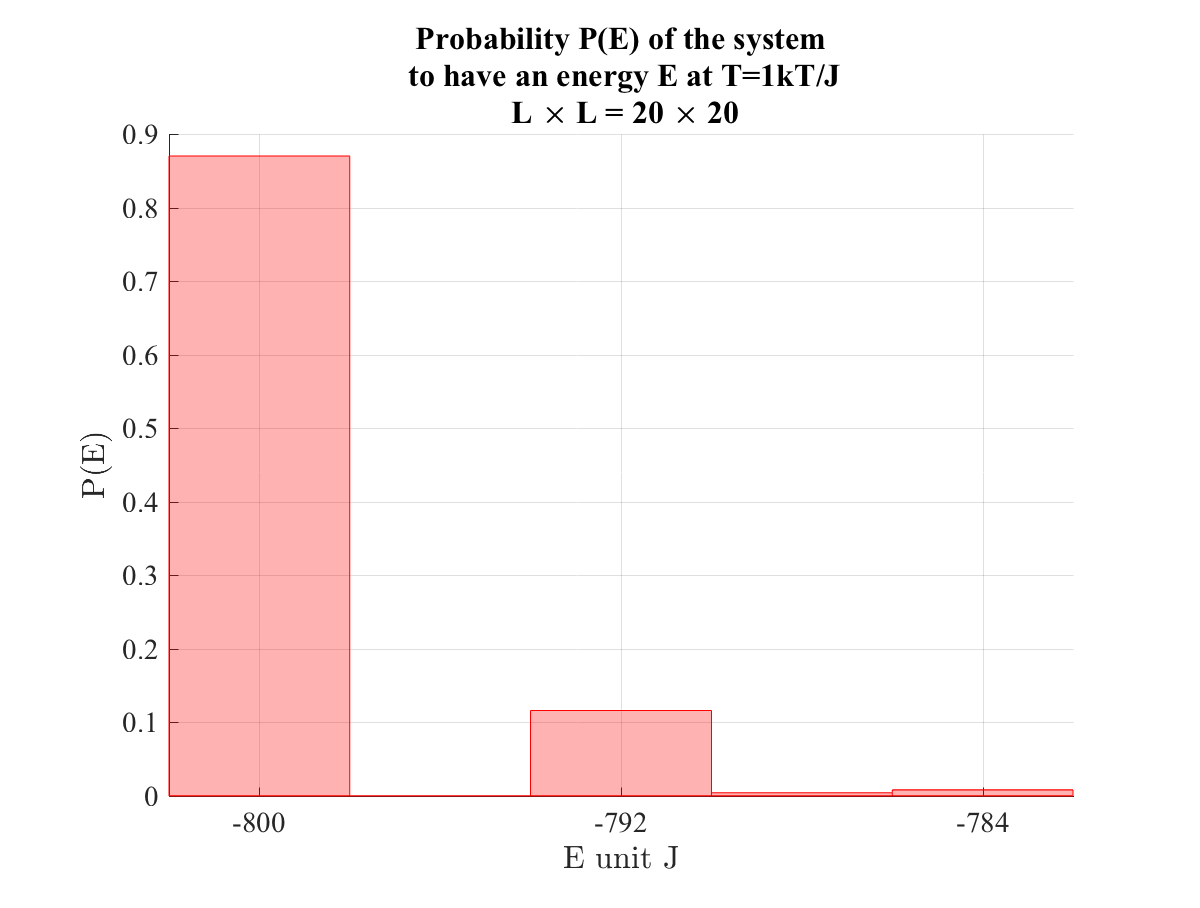
\includegraphics[scale=0.5]{pe20x20.eps}
\caption{The histogram shows the probability density function $P(E)$ at temparature $1 kT/J$. Most of the configurations in the system are in the lowest energy, due to the Boltzmann factor.}
\label{pe20x20}
\end{figure}
For $T=1 \, kT/J$ the histogram in Figure(\ref{pe20x20}) shows that more than $85 \%$ configurations assumes the lowest energy state. There is a very small likelihood for the system to pass to a bigger energy configuration because of the factor $\exp(-\Delta E/1J)$. Figure(\ref{acceptedconf}) shows the number of the accepted configurations $N_A$ as a function of the Monte Carlo cycles $n$. We have different slopes per each temperature.
\begin{figure}[h]
\centering
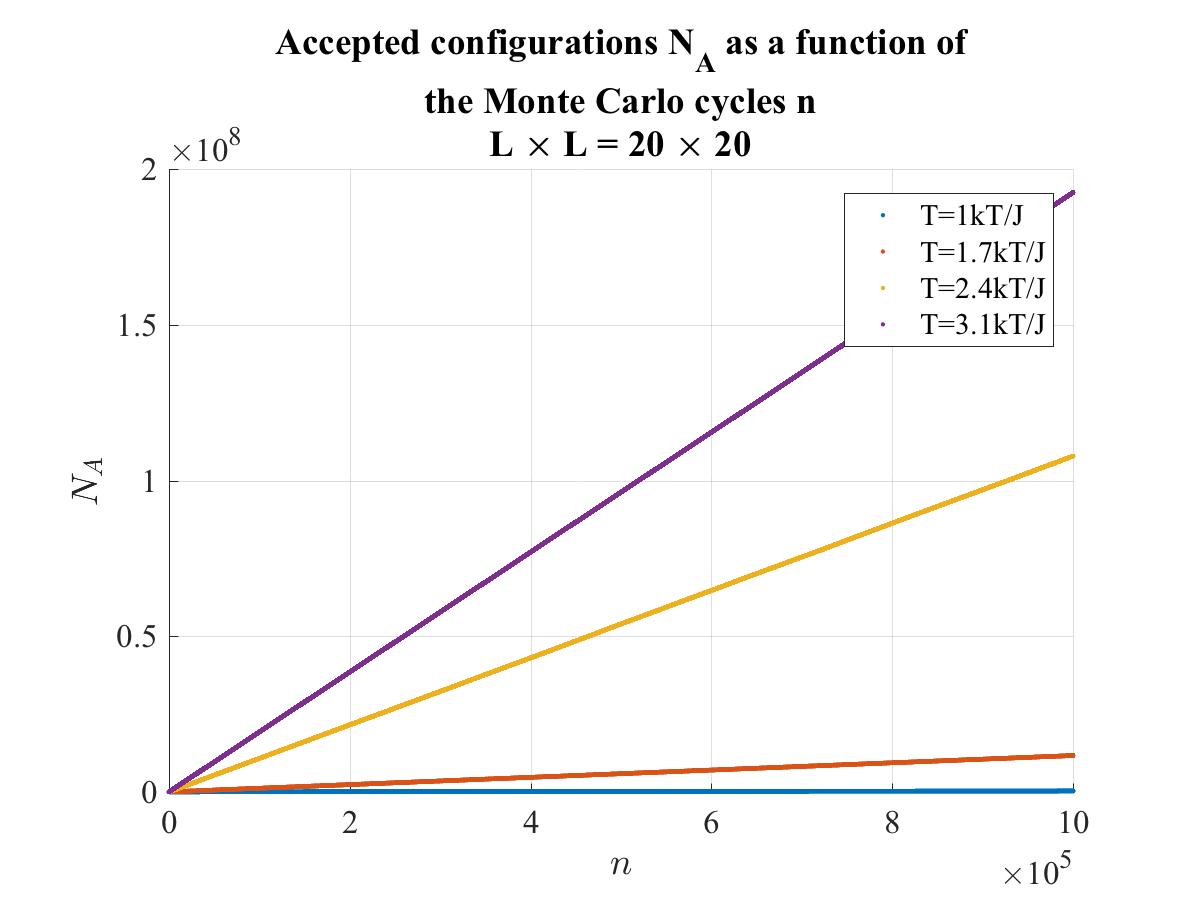
\includegraphics[scale=0.5]{acceptedconf.eps}
\caption{The accpeted configurations $N_A$ shows a linear behavior with a slope that increases with the temperature.}
\label{acceptedconf}
\end{figure}
Let us consider a difference between two energy configurations $\Delta E=4J$, so the boltzmann factor is $\approx 0.0183$. While if we increase the temperature up to $T= 1.7 kT/J$ we get a boltzmann factor five times bigger than before: $\approx 0.0951$ but with the same energy diference.
\begin{center}
\begin{figure}[h]
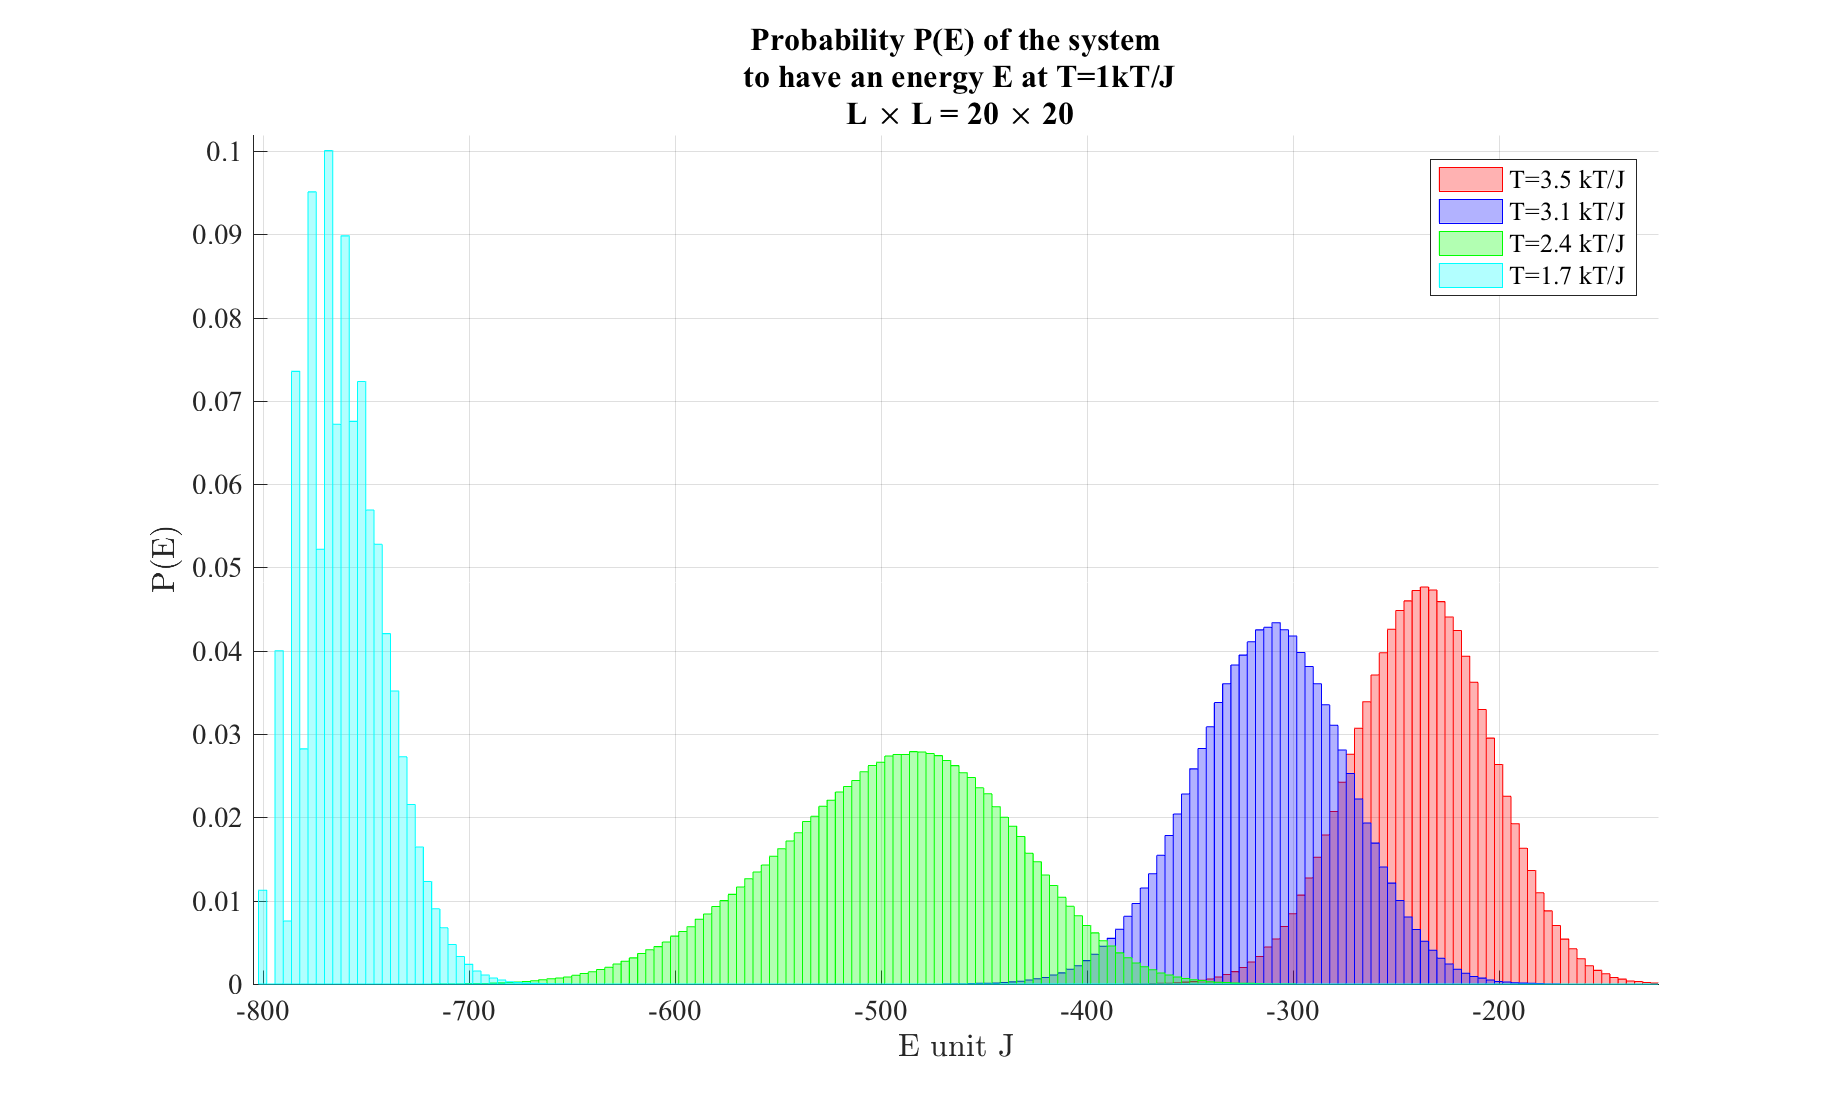
\includegraphics[scale=0.55]{pet20x20.eps}
\caption{This figure shows the different  energy distributions of our system at different temperatures. The behavior of $P(E)$ reflects the Boltzmann distribution.}
\label{pet20x20}
\end{figure}
\end{center}
In Figure(\ref{pet20x20}) is shown $P(E)$ for different temperatures. As we increase the temperature, more configurations have a bigger likelihood to be assumed by the system. The mean values of these distributions increase with the temperature as expected (Table(\ref{configurations})). However the variance $\sigma^2 _E$ of $P(E)$ has different behavior.
\begin{table}
\centering
\setlength{\tabcolsep}{12pt}
\caption{It is shown how the expecatation value of the energy and its variance change with the temperature.}
\label{configurations}
\begin{tabular}{ccc}
\toprule
$T$ &  $<E>$ & $\sigma^2 _E$ \\
\midrule
1	&	-798.87	&	9.4 \\
1.7	&	-759.27 &	394.9\\
2.4	&	-494.45 &	3246.3\\
3.1	&	-311.68 &	1387.5 \\
3.5	&	-237.59 &	1136.4 \\
\bottomrule
$kT/J$ & $J$ & $J^2$
\end{tabular}

\end{table}
At low temperatures the variance increases with the temperature, while at high temperatures we have the opposite behavior. The flattest probability density functions is at $T=2.4 kT/J$. To explain this we need to introduce the Helmholtz’ free energy.
\begin{equation}
\label{helmoltze}
F = <E> - \, T \, S = -k_B T \, \ln(Z)
\end{equation}
where $S$ is the entropy of the system, and it can be interpreted as the degree of disorder of our system. It can be shown that at the equilibrium $F$ has its minimum. 
Perhaps, Helmholtz’ free energy strikes a balance between the the minimum energy and the entropy increasing. 
For low temperatures most of the spins are aligned this implies a low entropy, so the minimum of $F$ is reached with the minimum of the energy. For high temperatures the spins are not aligned anymore in a specific direction the term $T \, S$ determines the behavior of $F$. For $T=2.4 \, kT/J$ we are close to the critical temperature of the system this leads to a flatter prbability distribution and high $\sigma^2_E$ because the system is in a transition phase. So the system takes more time before reaching the most likely energy. \\
With an infinitely large lattice if the system approaches to the critical temperature, $C_v$ and $\chi$ diverge.\\
\begin{figure}[h!]
\centering
     \subfloat[]{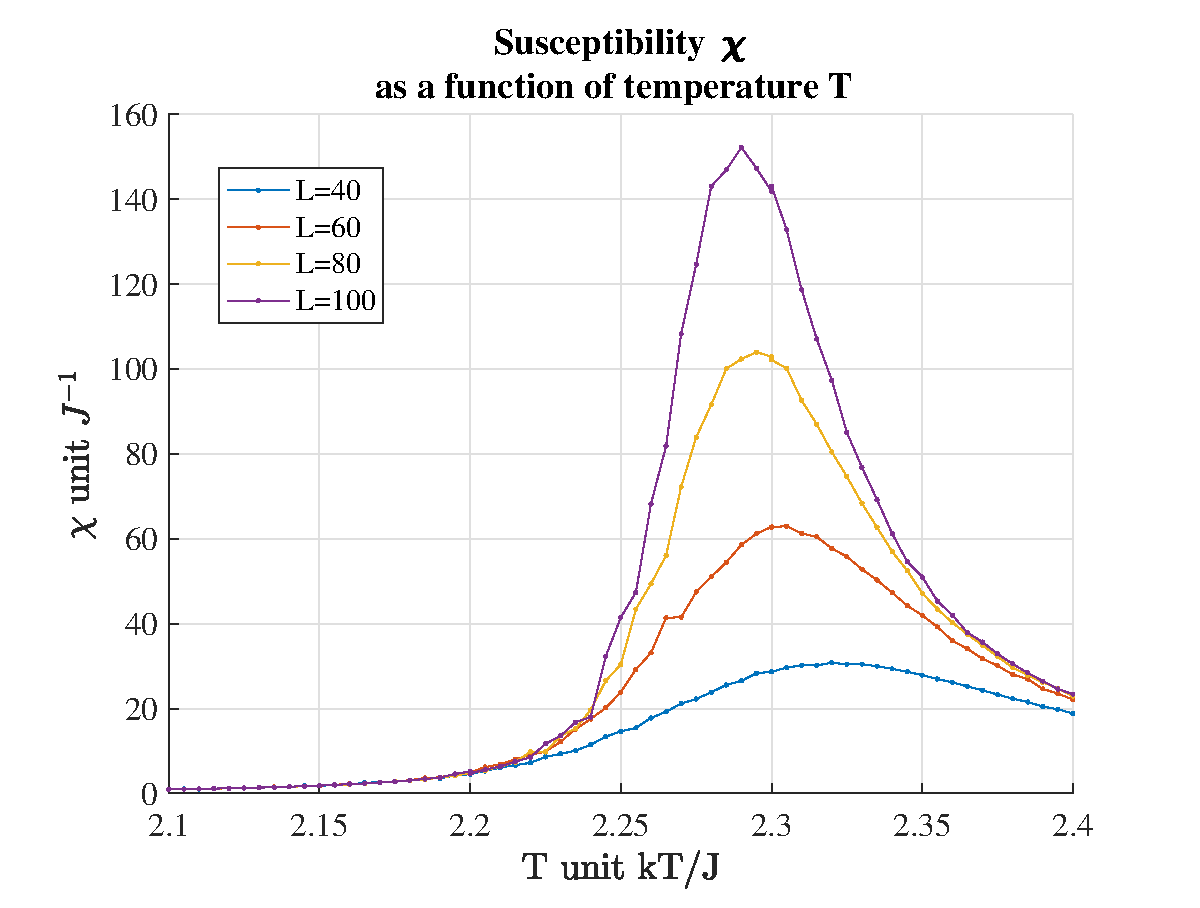
\includegraphics[width=.5\linewidth]{tcchi.eps}\label{tcchi}}
     \subfloat[]{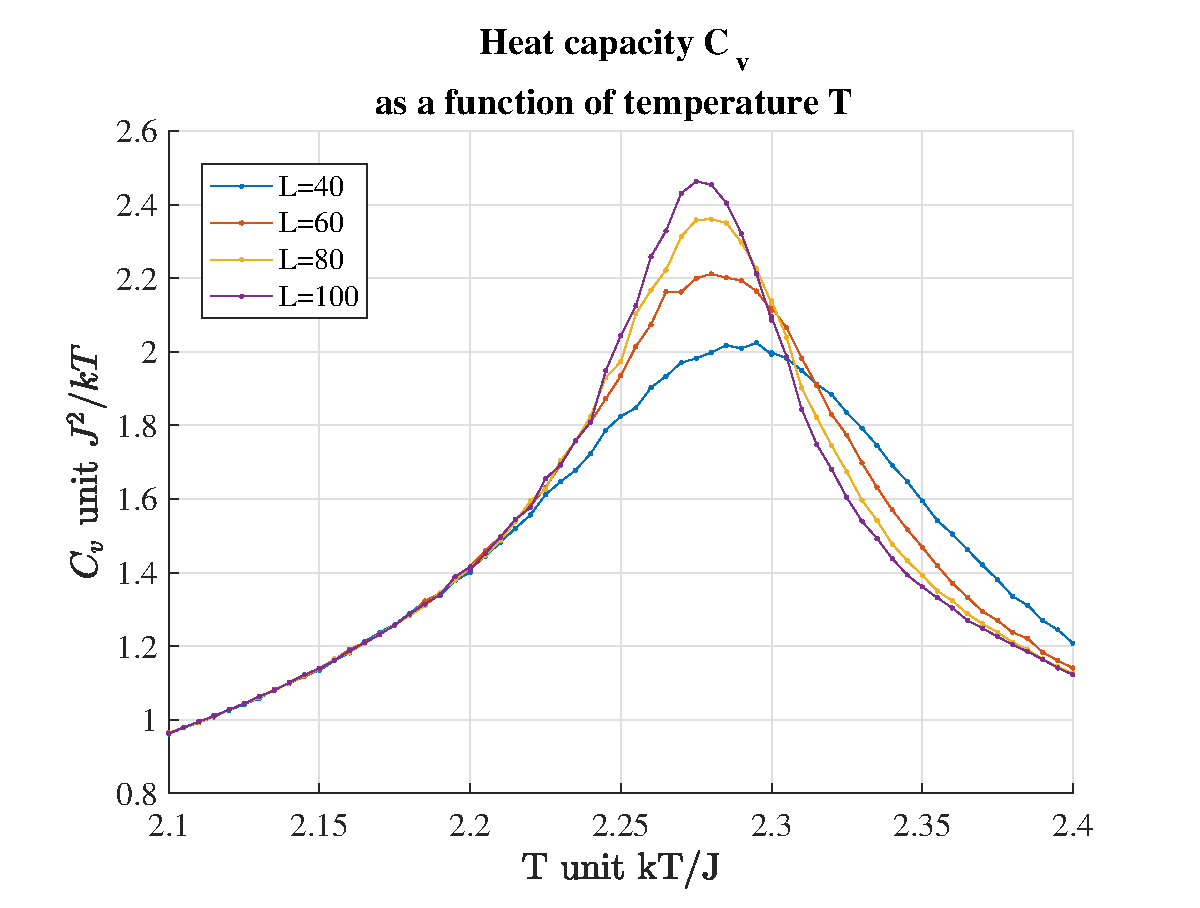
\includegraphics[width=.5\linewidth]{tccv.eps}\label{tccv}}
\caption{It is shown the behavior of heat capacity and suscepibility with different lattice dimension. The maximum of both the curves approaches to the thermodynamical limit $2.269$ when $L \to \infty$}
\end{figure}
Using this fact we simulate a phase transition increasing the temperature from $T=1 \, kT/J$ up to $T=2 \, kT/J$. Taking into account the previous discussion about the stability we run our program with the following definition of susceptibility:
\begin{equation}
\chi = <M^2>-<|M|>^2
\end{equation}
This definition is useful from a numerical point of view because it elimanates a lot of fluctuations. We also use calculate all the quantities per unit of spin.
We perform $n=10^6$ Monte Carlo cycles parallelizing the code on $8$ processors. 
Since we consider a finite lattice with $L=40,\,60,\, 80,\,100$ the calculated heat capacity and susceptibility will not exhibit a discontinuity but a broad maximum. We extract two critical temperatures $T_C ^{C_v}$ and $T_C ^{\chi}$ per each $L$ from the analysis of $C_v$ and $\chi$ in Figures (\ref{tccv}) and (\ref{tcchi}).  In Table (\ref{critict}) is shown that $T_C ^{C_v}$ and $T_C ^{\chi}$ decrease as $L$ increases.
\begin{table}
\centering
\setlength{\tabcolsep}{12pt}
\caption{It is shown the critical temperature obtained by the analysis of the heat capacity and susceptibility for different lattice size.}
\label{critict}
\begin{tabular}{ccc}
\toprule
$L$ & $T_C ^{C_v}$ & $T_C ^{\chi}$ \\
\midrule
 40 &  2.295 & 2.32 \\
 60 &  2.28 & 2.28  \\
  80 & 2.28  & 2.28   \\
 100 &  2.275 & 2.275 \\
\bottomrule
 & $kT/J$ & $kT/J$ \\ 
\end{tabular}

\end{table} In fact, Lars Onsager calculated the exact result of the critical temperature $T_C = 2/\ln(1 + \sqrt{2}) \approx 2.269$ for a two-dimensional infinite lattice (Ising model)[1]. To get a better result, the simulation should be run with a bigger value of the lattice dimension $L$, on the other hand, this leads to increase the running time.
We analyze mean energy and mean abslolute value of magnetization as a function of temperature Figures(\ref{tce}) and (\ref{tcabsm}). The energy increases while the magnetization tends to zero  as temperature increases. This opposite behavior reflects the fact that heating up the system we increase the energy of it but also the disorder and so entropy. As a consequence the spins they are free to be not aligned anymore and this leads $<|M|>$ to decreas. This is almost what happens when a ferromagnetic materials gets close to the Curie temperature.
\begin{figure}[h!]
     \subfloat[]{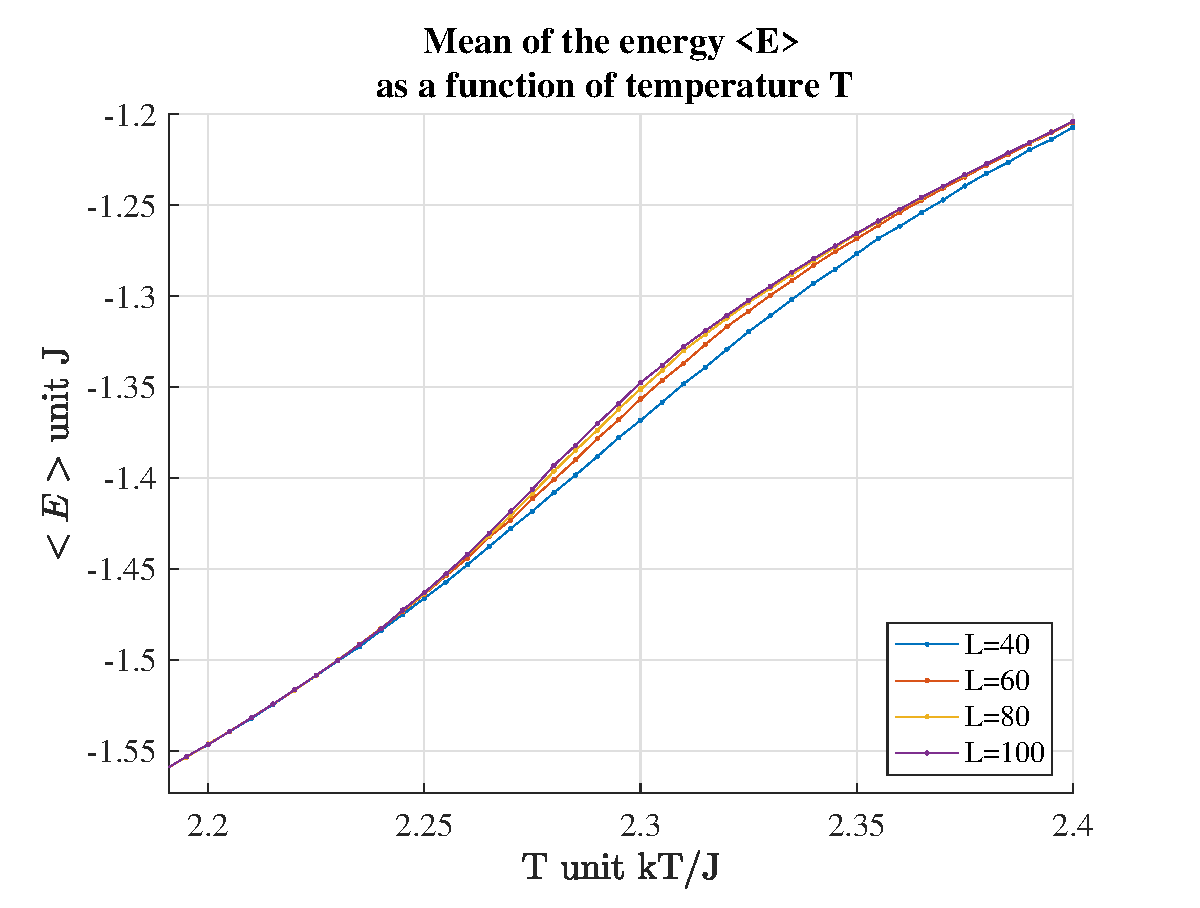
\includegraphics[width=.5\linewidth]{tce.eps}\label{tce}}
     \subfloat[]{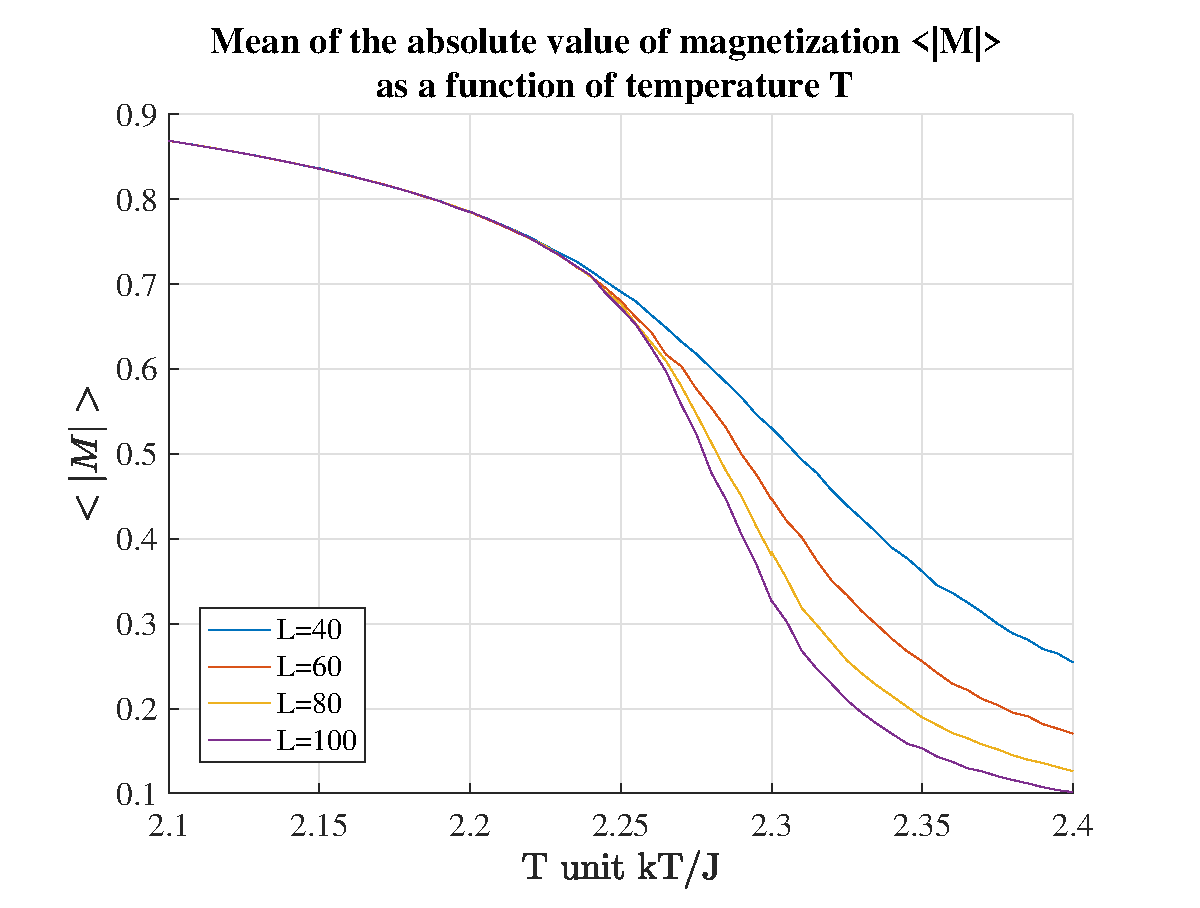
\includegraphics[width=.5\linewidth]{tcabsm.eps}\label{tcabsm}}
\caption{The mean energy of the system has a slightly largee value as $L$ increases. The mean of the absolute value decreases faster when $L$ is higher near the critical temperature.}
\end{figure}
\section{Conclusion}
%State your main findings and interpretations
%Try as far as possible to present perspectives for future work
%Try to discuss the pros and cons of the methods and possible improvements
We have seen that the system reaches an equilibrium state after  aproximately $n \approx 10^4$ Monte Carlo cycles for all temperatures. When the system has a temperature close to the critical temperature it takes more cycles $n$ before reaching a stable state.
The probability distribution of the energy $P(E)$  for $L=20$ is particularly narrow for low temperature. Thus the system has few possible energies that can acces, so indeed the variance is very small. On the other hand when $T$ is big the energy increases its value and the system can access more configurations thanks to the bigger Boltzmann factor $T >> 1 \Rightarrow \exp(-E/(k_B T)) \to 1$. \\
The heat capacity and the susceptibility show that clearly there is a phase transtion. Using this aspect we estimated a critical temperature $T_C = 2.275 kT/J$ for $L=100$. This confirms also that that the dimension of the lattice is not enough big to approximate the limit $L \to \infty$.
We can make an analogy thinking about a crystal formation. When the temperature is decreased slowly enough the atoms have time to organize in a specific structure that minimizes their energy. This process starts from a disordered configurations of the atoms and ends with a specific pattern of representing the entire solids.  
We can compare it to the degrees of freedom of atoms in a crystal with the alignment of the spins. Just as the atoms tend to be in a specific pattern , in our model when the temperature is decreased the spins allign themselves.
The main aspect of this project is that the using a quite simple model we are able to link the configurations of a system with the physical observables. In fact, statistical physics bridges the gap between the microscopic world and the macroscopic world.




%\section{Acknowledgments}
% \section{\label{sec:level1}First-level heading}

% This sample document demonstrates proper use of REV\TeX~4.1 (and
% \LaTeXe) in mansucripts prepared for submission to APS
% journals. Further information can be found in the REV\TeX~4.1
% documentation included in the distribution or available at
% \url{http://authors.aps.org/revtex4/}.

% When commands are referred to in this example file, they are always
% shown with their required arguments, using normal \TeX{} format. In
% this format, \verb+#1+, \verb+#2+, etc. stand for required
% author-supplied arguments to commands. For example, in
% \verb+\section{#1}+ the \verb+#1+ stands for the title text of the
% author's section heading, and in \verb+\title{#1}+ the \verb+#1+
% stands for the title text of the paper.

% Line breaks in section headings at all levels can be introduced using
% \textbackslash\textbackslash. A blank input line tells \TeX\ that the
% paragraph has ended. Note that top-level section headings are
% automatically uppercased. If a specific letter or word should appear in
% lowercase instead, you must escape it using \verb+\lowercase{#1}+ as
% in the word ``via'' above.

% \subsection{\label{sec:level2}Second-level heading: Formatting}

% This file may be formatted in either the \texttt{preprint} or
% \texttt{reprint} style. \texttt{reprint} format mimics final journal output. 
% Either format may be used for submission purposes. \texttt{letter} sized paper should
% be used when submitting to APS journals.

% \subsubsection{Wide text (A level-3 head)}
% The \texttt{widetext} environment will make the text the width of the
% full page, as on page~\pageref{eq:wideeq}. (Note the use the
% \verb+\pageref{#1}+ command to refer to the page number.) 
% \paragraph{Note (Fourth-level head is run in)}
% The width-changing commands only take effect in two-column formatting. 
% There is no effect if text is in a single column.

% \subsection{\label{sec:citeref}Citations and References}
% A citation in text uses the command \verb+\cite{#1}+ or
% \verb+\onlinecite{#1}+ and refers to an entry in the bibliography. 
% An entry in the bibliography is a reference to another document.

% \subsubsection{Citations}
% Because REV\TeX\ uses the \verb+natbib+ package of Patrick Daly, 
% the entire repertoire of commands in that package are available for your document;
% see the \verb+natbib+ documentation for further details. Please note that
% REV\TeX\ requires version 8.31a or later of \verb+natbib+.

% \paragraph{Syntax}
% The argument of \verb+\cite+ may be a single \emph{key}, 
% or may consist of a comma-separated list of keys.
% The citation \emph{key} may contain 
% letters, numbers, the dash (-) character, or the period (.) character. 
% New with natbib 8.3 is an extension to the syntax that allows for 
% a star (*) form and two optional arguments on the citation key itself.
% The syntax of the \verb+\cite+ command is thus (informally stated)
% \begin{quotation}\flushleft\leftskip1em
% \verb+\cite+ \verb+{+ \emph{key} \verb+}+, or\\
% \verb+\cite+ \verb+{+ \emph{optarg+key} \verb+}+, or\\
% \verb+\cite+ \verb+{+ \emph{optarg+key} \verb+,+ \emph{optarg+key}\ldots \verb+}+,
% \end{quotation}\noindent
% where \emph{optarg+key} signifies 
% \begin{quotation}\flushleft\leftskip1em
% \emph{key}, or\\
% \texttt{*}\emph{key}, or\\
% \texttt{[}\emph{pre}\texttt{]}\emph{key}, or\\
% \texttt{[}\emph{pre}\texttt{]}\texttt{[}\emph{post}\texttt{]}\emph{key}, or even\\
% \texttt{*}\texttt{[}\emph{pre}\texttt{]}\texttt{[}\emph{post}\texttt{]}\emph{key}.
% \end{quotation}\noindent
% where \emph{pre} and \emph{post} is whatever text you wish to place 
% at the beginning and end, respectively, of the bibliographic reference
% (see Ref.~[\onlinecite{witten2001}] and the two under Ref.~[\onlinecite{feyn54}]).
% (Keep in mind that no automatic space or punctuation is applied.)
% It is highly recommended that you put the entire \emph{pre} or \emph{post} portion 
% within its own set of braces, for example: 
% \verb+\cite+ \verb+{+ \texttt{[} \verb+{+\emph{text}\verb+}+\texttt{]}\emph{key}\verb+}+.
% The extra set of braces will keep \LaTeX\ out of trouble if your \emph{text} contains the comma (,) character.

% The star (*) modifier to the \emph{key} signifies that the reference is to be 
% merged with the previous reference into a single bibliographic entry, 
% a common idiom in APS and AIP articles (see below, Ref.~[\onlinecite{epr}]). 
% When references are merged in this way, they are separated by a semicolon instead of 
% the period (full stop) that would otherwise appear.

% \paragraph{Eliding repeated information}
% When a reference is merged, some of its fields may be elided: for example, 
% when the author matches that of the previous reference, it is omitted. 
% If both author and journal match, both are omitted.
% If the journal matches, but the author does not, the journal is replaced by \emph{ibid.},
% as exemplified by Ref.~[\onlinecite{epr}]. 
% These rules embody common editorial practice in APS and AIP journals and will only
% be in effect if the markup features of the APS and AIP Bib\TeX\ styles is employed.

% \paragraph{The options of the cite command itself}
% Please note that optional arguments to the \emph{key} change the reference in the bibliography, 
% not the citation in the body of the document. 
% For the latter, use the optional arguments of the \verb+\cite+ command itself:
% \verb+\cite+ \texttt{*}\allowbreak
% \texttt{[}\emph{pre-cite}\texttt{]}\allowbreak
% \texttt{[}\emph{post-cite}\texttt{]}\allowbreak
% \verb+{+\emph{key-list}\verb+}+.

\section{Bibliography}
\begin{itemize}
\item[[1]] Lars Onsager, \textit{Crystal Statistics. I. A Two-Dimensional Model with an Order-Disorder Transition}, 1 February 1944
\item M. H. Jensen, \textit{Computational physics - Lecture notes Fall 2015}, University of Oslo - Department of Physics, 2015. 
\item https://i.stack.imgur.com/CCS4m.png.

\end{itemize}





%










%. Thermodynamical quantities such as the specific heat or net magnetization of a system can all be derived from a microscopic theory
%In statistical mechanics, a canonical ensemble is the statistical ensemble that represents the possible states of a mechanical system in thermal equilibrium with a heat bath at a fixed temperature.[1] The system can exchange energy with the heat bath, so that the states of the system will differ in total energy
% derivation from canonical ensemble https://en.wikipedia.org/wiki/Maxwell–Boltzmann_statistics
\end{document}
